% Chapter 9

\chapter{Classification} % Main chapter title

\label{Chapter9} % For referencing the chapter elsewhere, use \ref{Chapter1} 

Since most preprocessing required for classification here had already been performed in the first task of the project, I did not feel the need to conduct it again and simply re-used the dataset at the standardization stage. So, this is a sample of the DataFrame I started working with:

\begin{figure}[h]
    \centering
    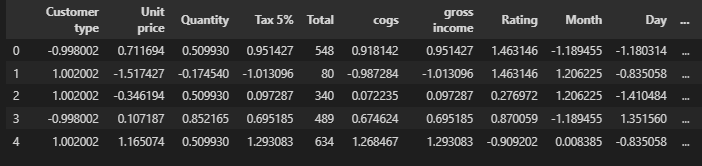
\includegraphics[width=1\textwidth]{Chapters/ch9/data_1.png}
    % \caption{This is an example image.}
    % \label{fig:example}
\end{figure}

\lhead{Chapter 9. \emph{Classification}} % This is for the header on each page - perhaps a shortened title

%----------------------------------------------------------------------------------------

\section{Choosing the Target Variable:}

 In the context of our problem (Customer Segmentation), the target variable was a choice between 2 features. Although other features could also be utilized, these 2 features seemed the best for performing customer segmentation. The 2 features are ‘Total’ and ‘Customer type’. 
 \newline 
 I chose ‘Total’ due to its direct relevance to overall customer spending. It encapsulates the comprehensive financial transaction for each customer, making it a meaningful and practical variable for segmentation. The choice is justified by the potential predictive power of variations in spending patterns, the business relevance of understanding different customer segments, and the ability to employ classification metrics for model evaluation. Furthermore, the interpretability of 'Total' spending segments enhances the practical impact on business decision-making, aligning with the overarching goal of gaining actionable insights into customer behavior.
 \newline
 ‘Customer type’, on the other hand, enables the model to differentiate between distinct customer types, such as "Member" and "Normal," offering valuable information for targeted marketing strategies, loyalty programs, and operational decision-making. Predicting customer types can aid in customer retention efforts and enhance the overall customer experience by tailoring services to the specific needs and expectations of different segments. 
 \newline 
 Hence, from a business as well as a technical perspective (applying models), both features seem to make a lot of sense as the target variable. As I mentioned before, there are other features that could be used for this task as well. These include Product line, Payment Method, and Quantity. For customer segmentation specifically however, I felt ‘Total’ and ‘Customer type’ made more sense.
 \newline
 I chose ‘Total’ from these two because I wanted to explore the concept and application of binning. As ‘Total’ is a continuous feature and ‘Customer type’ is categorical.
\newline 
By this point, I had cleaned, encoded, and standardized the data. However, binning was required before splitting the data, since my chosen target variable was ‘Total’, and this is a continuous feature in the dataset.

\section{Binning:}

\subsection{The concept of binning:}
Binning, also known as discretization, is a data preprocessing technique commonly used in data analysis and machine learning to handle numerical data. The general logic behind binning is to simplify the data and make it more manageable, especially when dealing with continuous variables. This process involves grouping a range of continuous or numerical data points into a smaller number of discrete "bins" or intervals.

\subsection{Choosing an ideal number of bins:}
For this step, I decided to use various rules which help indicate the ideal value for bins to use.

\subsubsection{Square Root Rule:}
This is a simple method that calculates the number of bins by taking the square root of the total number of data points in the dataset. The formula is usually given as sqrt(n), where 'n' is the number of data points. It is easy to apply and works well for datasets of various sizes. It helps in preventing the creation of too many or too few bins.

\subsubsection{Sturges’ Formula:}
\begin{equation}
k = 1 + \log^2(N)
\end{equation}
where:
\begin{itemize}
\item k is the number of bins.
\item N is the number of data points.
\end{itemize}

This formula assumes that the data follows a normal distribution. It is widely used and is suitable for datasets with a normal distribution. However, it may not perform well for datasets with outliers or non-normal distributions.

\subsubsection{Scott’s Rule:}
\begin{equation}
3.5 * (S.D.) * (n^(-1/3))
\end{equation}
where:
\begin{itemize}
\item h is the bin width.
\item N is the number of data points.
\end{itemize}

This rule considers the variability of the data.
It is robust and performs well for datasets with varying degrees of variability. It adapts to the distribution of the data and is less sensitive to outliers.

\subsubsection{Freedman-Diaconis Rule:}
\begin{equation}
2 * IQR * (n^(-1/3))
\end{equation}
where:
\begin{itemize}
\item h is the bin width.
\item IQR is the interquartile range.
\item N is the number of data points.
\end{itemize}
This rule is particularly useful when dealing with datasets with outliers. It adjusts the bin width based on the spread of the data, making it less sensitive to extreme values.

\subsubsection{Doane’s Formula:}
\begin{equation}
    1 + log2(n) + log2(1 + |g1|/sigma_g1)
\end{equation}
where:
\begin{itemize}
\item k is the number of bins.
\item N is the number of data points.
\item g1 is the skewness of the data.
\item sigma(g1) is the standard error of the skewness.
\end{itemize}

This Formula is an extension of Sturges' Formula that also considers the skewness of the data. It is suitable for datasets with non-normal distributions and can provide a more accurate estimate of the number of bins when skewness is present.

\subsubsection{Results}
Here are all the results summarized:
\begin{table}[htbp]
    \centering
    \begin{adjustbox}{max width=\textwidth} % Fit the table to the page width
        \rowcolors{1}{green!20}{white} % Alternate row colors starting from the second row
        \rowcolors{2}{green!30}{white} % Slightly darker header row
        \begin{tabular}{|>{\columncolor{green!50}}c|c|}
            \hline
            \rowcolor{green!50} % Slightly darker header row color
            \textbf{Method} & \textbf{Number of Bins} \\
            \hline
            Square Root Rule  & 31 \\
            Sturges' Formula  & 11 \\
            Scott's Rule & 11 \\
            Freedman-Diaconis Rule & 14 \\
            Doane's Formula & 13 \\
            \hline
        \end{tabular}
    \end{adjustbox}
    % \caption{3 x 2 Table with alternating light green rows and a slightly darker green header}
    \label{tab:3x2_table}
\end{table}


Thus, from these results, the bin values were tending towards a value around 12. However, upon using such several bins, I faced issues. Hence, I went back to conduct further analysis:


\begin{figure}[h]
    \centering
    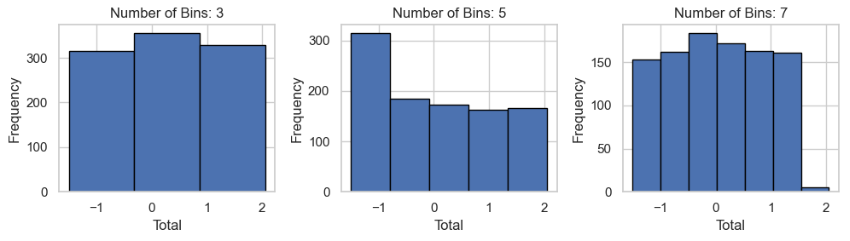
\includegraphics[width=0.7\textwidth]{Chapters/ch9/binning-1.png}
    % \caption{Radar graph}
    % \label{fig:example}
\end{figure}
\begin{figure}[h]
    \centering
    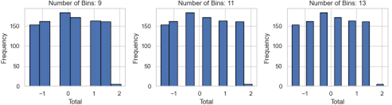
\includegraphics[width=0.7\textwidth]{Chapters/ch9/bar_chart_2.png}
    % \caption{Radar graph}
    % \label{fig:example}
\end{figure}

As can be seen from these graphs, a higher value for the bins seems to form a sparser distribution. Thus, we might want to use a lower number of bins.

\begin{figure}[h]
    \centering
    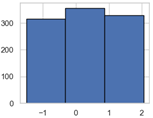
\includegraphics[width=0.2\textwidth]{Chapters/ch9/bar_chart_3.png}
    % \caption{Radar graph}
    % \label{fig:example}
\end{figure}
Judging from this, I decided to choose the number of bins to be 3, which seemed to be the ideal value as can be seen by this graph. All 3 bars, each representing a discrete ‘Total’ value, have an almost equal number of frequencies in our dataset. 


\subsection{Deciding on the bin edges:}
Once I decided how many bins to use, the next step was figuring out what values were to be assigned to these bins. Let me explain. I chose the number of bins for ‘Total’ to be 3. Which means that the ‘Total’ column will be discretized into 3 categories. But on what basis? How will we decide what value the original ‘Total’ goes into which bin? For this, I explored our data some more:
\newline
\newline
As can be seen below, the count of the discrete values present in ‘Total’ is 546:
\newline
Total
\newline
125    6
\newline
175    6
\newline
      ..
\newline
721    1
\newline
149    1
\newline
649    1
\newline
Name: count, Length: 546, dtype: int64
\newline
Also note, the Variance of the column ‘Total’ is 60457.8.
\newline 
\newline 
These values have given us an idea about the spread of the column ‘Total’. To understand this spread more, its evenness and unevenness, I used the following visualizations:
\begin{figure}[h]
    \centering
    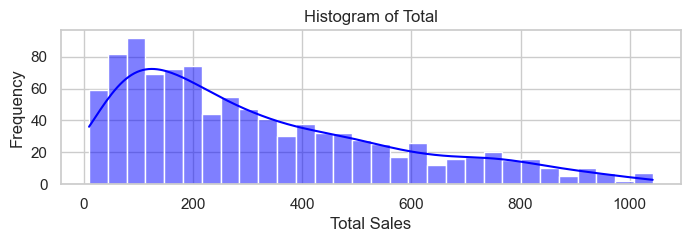
\includegraphics[width=0.5\textwidth]{Chapters/ch9/ch_9_hist.png}
    % \caption{Radar graph}
    % \label{fig:example}
\end{figure}
\begin{figure}[h]
    \centering
    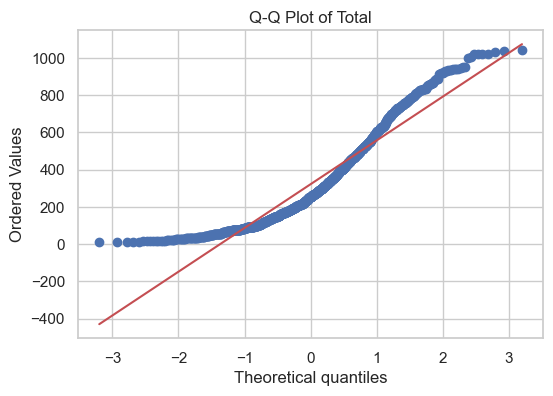
\includegraphics[width=0.5\textwidth]{Chapters/ch9/ch_9_linechart.png}
    % \caption{Radar graph}
    % \label{fig:example}
\end{figure}
As can be seen here, the blue line (actual values) does not follow a straight line, meaning the ‘Total’ column is not normally distributed. The points deviate from the line, especially towards the tails, which indicates a departure from normality. The points curving upwards and downwards suggest skewness or light/heavy-tailed distribution.
\newline
\newline
I made use of the ‘Quantile’ method to calculate the bin edges.  This method allows us to identify the values corresponding to specific percentiles within the distribution of the 'Total' column. I computed the 33rd and 66th percentiles, and the resulting values are utilized as reference points for defining the bin edges. Following is the code for this process:

\begin{lstlisting}[language=Python, frame=none]
percentile\_33 = df\_classif['Target'].quantile(0.33) 
percentile\_66 = df\_classif['Target'].quantile(0.66) 
bin\_edges = [df\_classif['Target'].min()
, percentile\_33, percentile\_66,df\_classif['Target'].max()] 
Bin Edges: 
[10, 163.0, 381.68000000000006, 1042]
\end{lstlisting}

\subsection{Applying binning:}
The last step before applying binning was to set the bin labels. I decided to set these to Low, Medium, and High. Since we’re applying binning on our ‘Total’ feature, which represents the total bill for each transaction, these labels seem to be good choices to categorize customer behavior.
\newline 
\newline
After this, I applied binning using our decided labels, edges, and number of bins:
\begin{lstlisting}[language=Python, frame=none]
df_classif['Total_bins'] = pd.cut(df_classif[column_name], bins=bin_edges, labels=bin_labels, include_lowest=True)
\end{lstlisting}
\newline 
\newline 
I made use of the powerful Pandas function ‘pd.cut’ to discretize the continuous feature ‘Total’. The first 3 parameters of the function are self-explanatory. The fourth parameter (include\_lowest) determines whether the leftmost edge of the bins should be considered as a valid bin edge or not. I’ve set this to true.
\newline 
\newline 
Here is the result following binning:
\newline 
0        High
\newline 
1         Low
\newline 
2      Medium
\newline 
3        High
\newline 
4        High
\newline 
        ...
\newline 
995       Low
\newline 
996      High
\newline 
997       Low
\newline
998       Low
\newline 
999      High
\newline 
Name: Total, Length: 1000, dtype: category
\newline 
Categories (3, object): ['Low' < 'Medium' < 'High']
\subsection{Analyzing ‘Total’ after binning:}

\begin{table}[htbp]
    \centering
    \begin{adjustbox}{max width=\textwidth} % Fit the table to the page width
        \rowcolors{1}{green!20}{white} % Alternate row colors starting from the second row
        \rowcolors{2}{green!30}{white} % Slightly darker header row
        \begin{tabular}{|>{\columncolor{green!50}}c|c|}
            \hline
            \rowcolor{green!50} % Slightly darker header row color
            \textbf{Category} & \textbf{Frequency} \\
            \hline
            Low  & 331 \\
            Medium  & 329 \\
            High & 340 \\
            \hline
        \end{tabular}
    \end{adjustbox}
    % \caption{3 x 2 Table with alternating light green rows and a slightly darker green header}
    \label{tab:3x2_table}
\end{table}

In the above table, we can observe the frequencies of the new categories. Let’s visualize this using a histogram:
\begin{figure}[h]
    \centering
    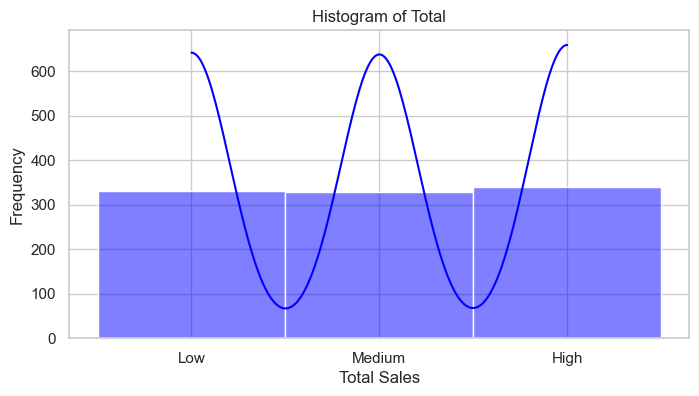
\includegraphics[width=0.5\textwidth]{Chapters/ch9/ch_9_w_graph.png}
    % \caption{Radar graph}
    % \label{fig:example}
\end{figure}
All 3 categories reach approximately equal highs and lows. This indicates that we have performed binning efficiently and can move onto the next step of the classification process.

\begin{figure}[h]
    \centering
    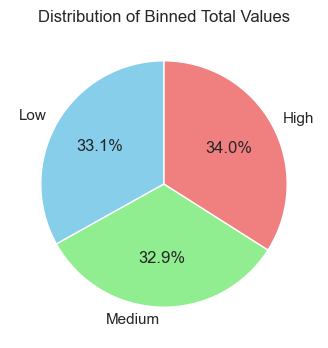
\includegraphics[width=0.3\textwidth]{Chapters/ch9/ch_9_piechart_1.png}
    % \caption{Radar graph}
    % \label{fig:example}
\end{figure}
This pie chart shows the spread of the categories High, Medium and Low as percentages of the ‘Total’ feature. It indicates that sampling is not required as these categories are roughly equal.

% ---------------------------------------------------------------------------------------------

\section{Splitting data }
Using Train-Test split, I split the dataset.  I already covered this step, in detail, during the preprocessing stage, so I won’t go into detail here.
\newline 
\newline 
Training set shape: (800, 22) (800,)
\newline 
Testing set shape: (200, 22) (200,)

% -----------------------------------------------------------------------------
\section{Model Training and Testing:}
Since the code after this is short, and applying the actual model is a small step, I decided to apply multiple models. Here are details about their obtained accuracy metrics:


\begin{table}[htbp]
    \centering
    \begin{adjustbox}{max width=\textwidth} % Fit the table to the page width
        \rowcolors{1}{green!20}{white} % Alternate row colors starting from the second row
        \rowcolors{2}{green!30}{white} % Slightly darker header row
        \begin{tabular}{|>{\columncolor{green!50}}c|c|c|c|c|}
            \hline
            \rowcolor{green!50} % Slightly darker header row color
            \textbf{Model} & \textbf{Accuracy} & \textbf{Precision} & \textbf{Recall} & \textbf{F1-Score} \\
            \hline
            \cellcolor{green!30}Random Forest  & 0.940 & 0.942260 &	0.940 &	0.940410\\
            \cellcolor{green!30}Gradient Boosting & 0.925 & 0.927232 &	0.925 & 0.925458 \\
            \cellcolor{green!30}Logistic Regression & 0.940	& 0.940435 & 0.940 & 0.939632 \\
            \cellcolor{green!30}Naive Bayes  & 0.920 & 0.921063 & 0.920 &	0.920297\\
            \cellcolor{green!30}K-Nearest Neighbors & 0.810	& 0.816504 &	0.810 &	0.812382 \\
            \cellcolor{green!30}Support Vector Machine & 0.915 & 0.914824 & 0.915 &	0.914877\\
            \hline
        \end{tabular}
    \end{adjustbox}
    % \caption{7 by 5 Table with alternating light green rows and a slightly darker green header}
    \label{tab:7x5_table}
\end{table}

\textbf{Key Findings:}
\begin{itemize}
\item Random Forest and Logistic Regression outperform other models with the highest accuracy of 94.0%.
\item Precision is consistently high across all models, indicating a low false positive rate in classifying customers.
\item Recall values are generally balanced, suggesting good performance in capturing true positive instances.
\item F1-Score combines precision and recall, showcasing the overall effectiveness of the model. Random Forest and Logistic Regression excel in this aspect.
\end{itemize}

\textbf{Conclusion}
Considering the high accuracy, precision, recall, and F1-Score, Random Forest or Logistic Regression is recommended for predicting customer segments based on purchasing behavior.




